%!TEX root = main.tex
\thispagestyle{firststyle}
%\pagestyle{fancy}
\title{Trabajo Final:\\Sistema de programación para estimulador basado en {ESP32s}}
\author{Esteban Osella}
\maketitle
\thispagestyle{firststyle}
%\shorthandoff{>}\shorthandoff{<}
%\newpage \pagenumbering{arabic}

%\thispagestyle{empty}
\onehalfspace
%\begin{figure}[htb]
	%\centering
		%\includegraphics[width=0.5\paperwidth]{figs/mesa_optica.jpg}
		%\caption{Dinamómetro}
	%\label{fig:mesa_optica}
%\end{figure}	
\section{Planteo del problema}
En el “Laboratorio de Ingeniería en Rehabilitación e Investigaciones Neuromusculares y Sensoriales (LIRINS)” de la FI-UNER se cuenta con un prototipo de estimulador eléctrico funcional (FES), desarrollado por el propio laboratorio. El estimulador se comanda por intermedio de una placa ESP32s programada en arduino que permite determinar los parámetros de estimulación a través de bluetooth utilizando una aplicación desde un teléfono celular. 

Inicialmente, la aplicación en cuestión fue programada (en el contexto de un proyecto final de grado) mediante la herramienta \href{http://ai2.appinventor.mit.edu/}{appInventor}, la cual provee un entorno de programación visual muy amigable, como se aprecia en \ref{fig:primer_prototipo}. Sin embargo, esta herramienta quedó sin soporte para versiones de Android posteriores a 5.1.1 (LMY49M) Lollipop. Surge entonces la necesidad de contar con una herramienta que permita tener una mayor flexibilidad con respecto a los dispositivos en los cuales se puede instalar la herramienta en cuestión. 

\begin{figure}[htb]
	\centering
		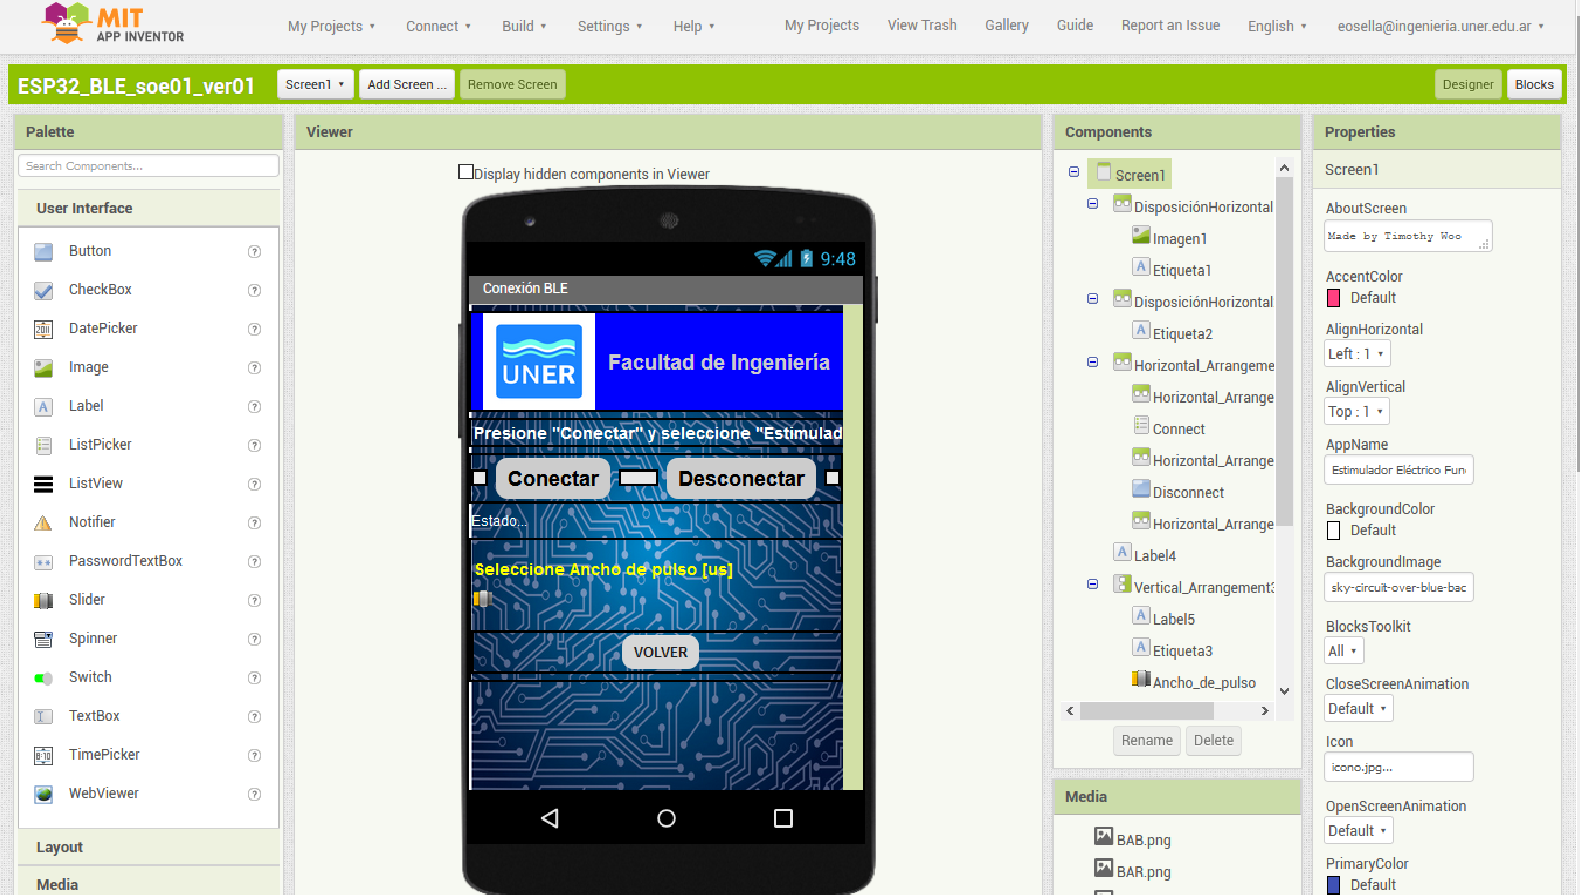
\includegraphics[width=1.00\textwidth]{figs/appInventor.png}
		\caption{Prototipo a reemplazar de la  aplicación.}
	\label{fig:primer_prototipo}
\end{figure}


\section{Solución planteada}
Como alternativa, se planteó una aplicación en ionic basado en el diseño de páginas con menú. En estas páginas encontramos:
\begin{itemize}
	\item \textit{Start:} una página de bienvenida, describiendo la aplicación (Figure \ref{fig:welcome}).
	\item \textit{Connect:} una página que busca los dispositivos bluetooth disponibles y establece la conexión, y el envío de la información al dispositivo (Figure \ref{fig:connections}).
	\item \textit{Stimulator Configuration:} página para configurar los parámetros máximos y mínimos, la identidad del paciente, la cantidad de canales, y, para futuro, la ip del servidor donde se podrían almacenar las configuraciones. 
	\item \textit{Channel setup:} página para determinar la configuración de cada canal. Permite también realizar pruebas en cada canal, sin necesariamente grabar dicha configuración en el estimulador (Figure \ref{fig:ch_setup}).
\end{itemize}
Para establecer la comunicación bluetooth entre los dispositivos se utiliza la biblioteca \href{https://ionicframework.com/docs/native/bluetooth-serial}{BluetoothSerial} en la aplicación, y \href{https://arduinojson.org/}{arduinojson} para la serialización y deserialización de la información en el dispositivo.

Se modeló cada canal y el estimulador con clases específicas y la interacción entre ellas se realizó mediante un servicio que las vincula, así como también para la validación de los límites de estimulación. En las clases correspondientes se implementaron métodos para la serialización de la información {JSON}. 

El código fuente del presente proyecto puede obtenerse en 

\href{https://github.com/osellaesteban/stimConfigurator}{https://github.com/osellaesteban/stimConfigurator}.

\begin{figure}
\begin{subfigure}{.5\textwidth}
  \centering
  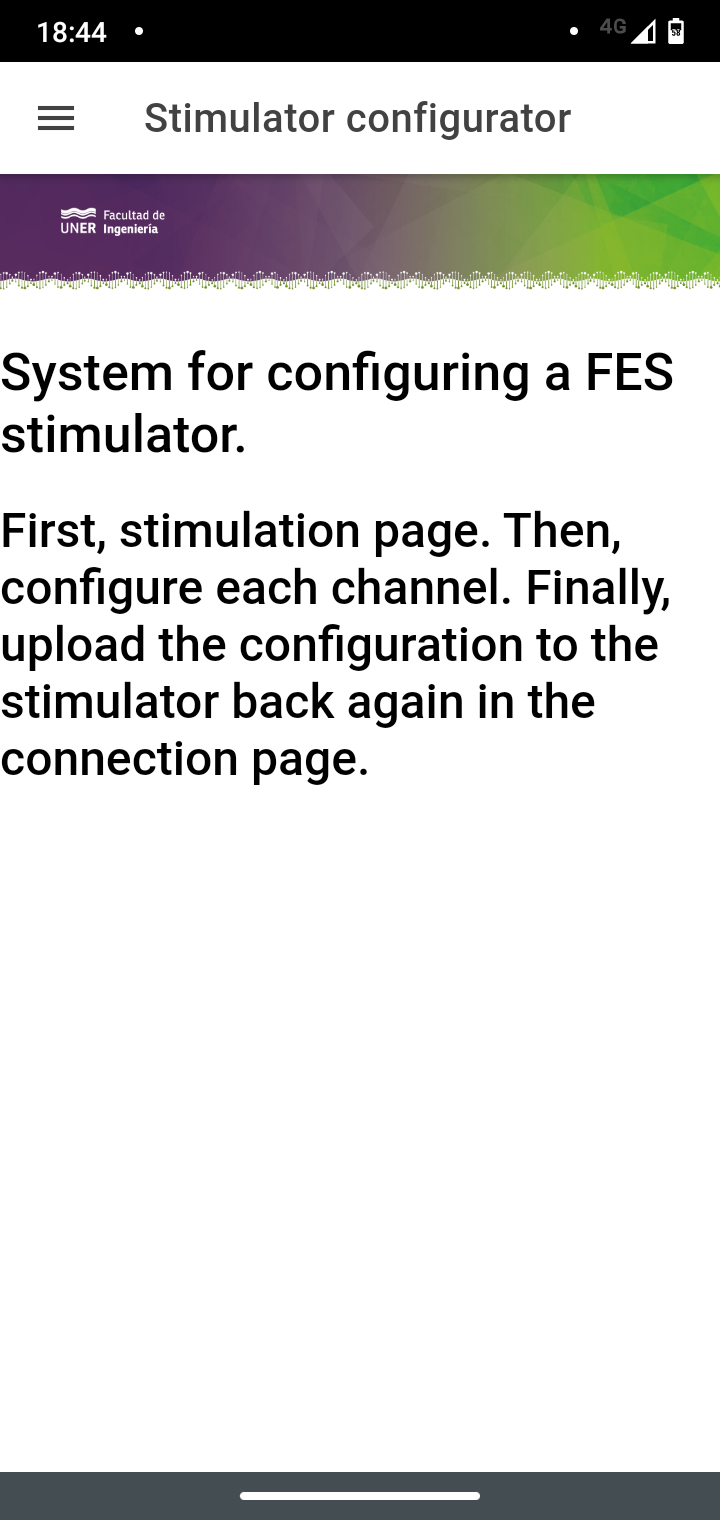
\includegraphics[width=.8\linewidth]{figs/01_start.png}
  \caption{Página de bienvenida}
  \label{fig:welcome}
\end{subfigure}%
\begin{subfigure}{.5\textwidth}
  \centering
  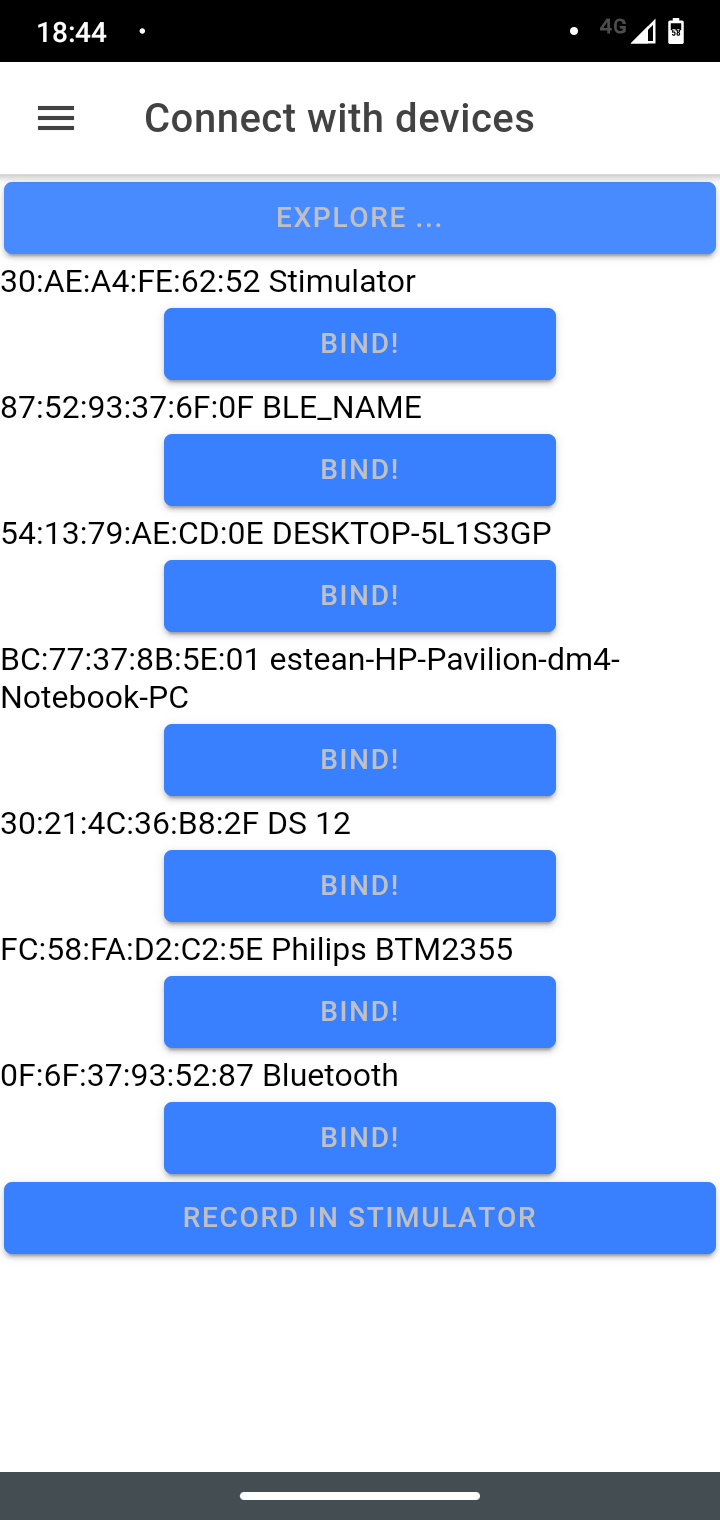
\includegraphics[width=.8\linewidth]{figs/02_connection.png}
  \caption{Página de conexiones}
  \label{fig:connections}
\end{subfigure}
\caption{Páginas de bienvenida y conexiones}
\label{fig:welcomeConnect}
\end{figure}
\begin{figure}
\begin{subfigure}{.5\textwidth}
  \centering
  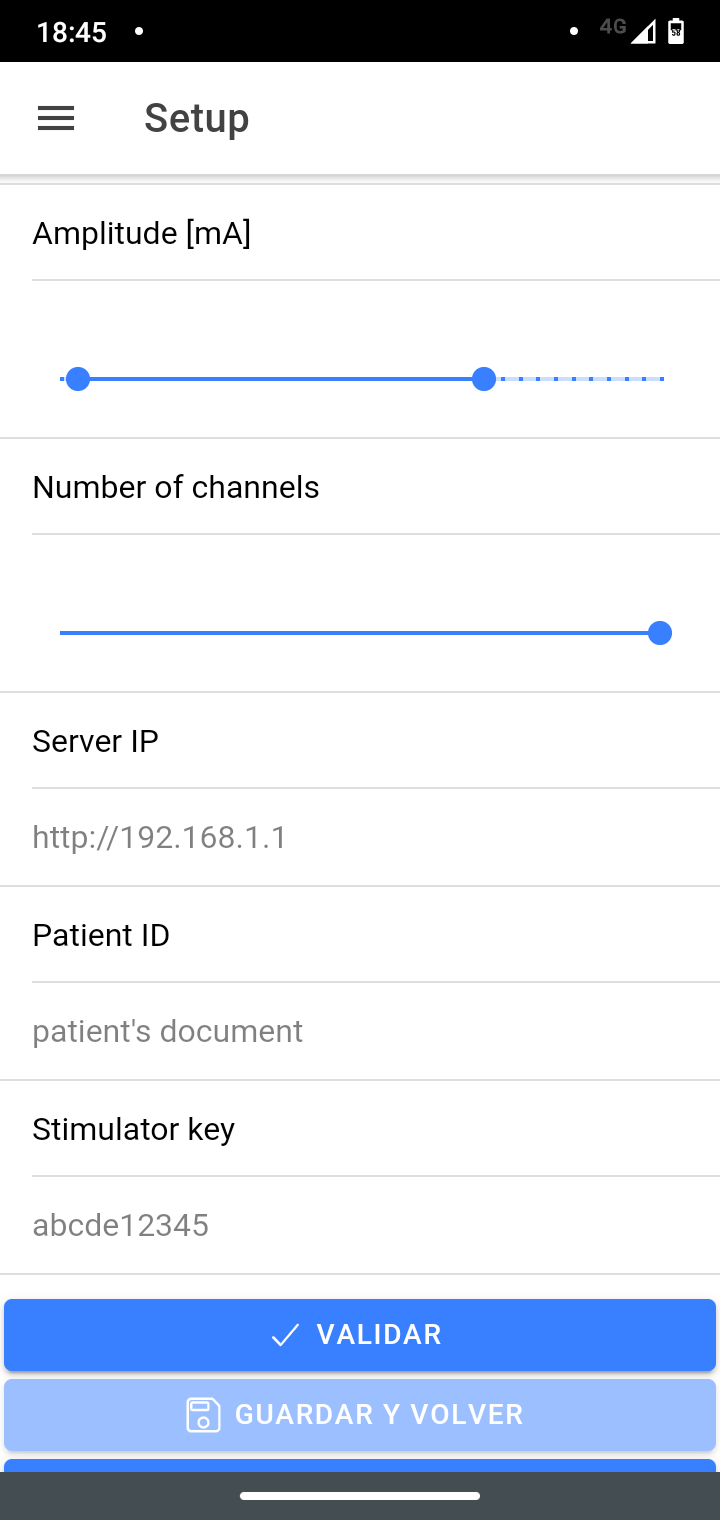
\includegraphics[width=.8\linewidth]{figs/03_setup.png}
  \caption{Configuración del estimulador.}
  \label{fig:setup}
\end{subfigure}
\begin{subfigure}{.5\textwidth}
  \centering
  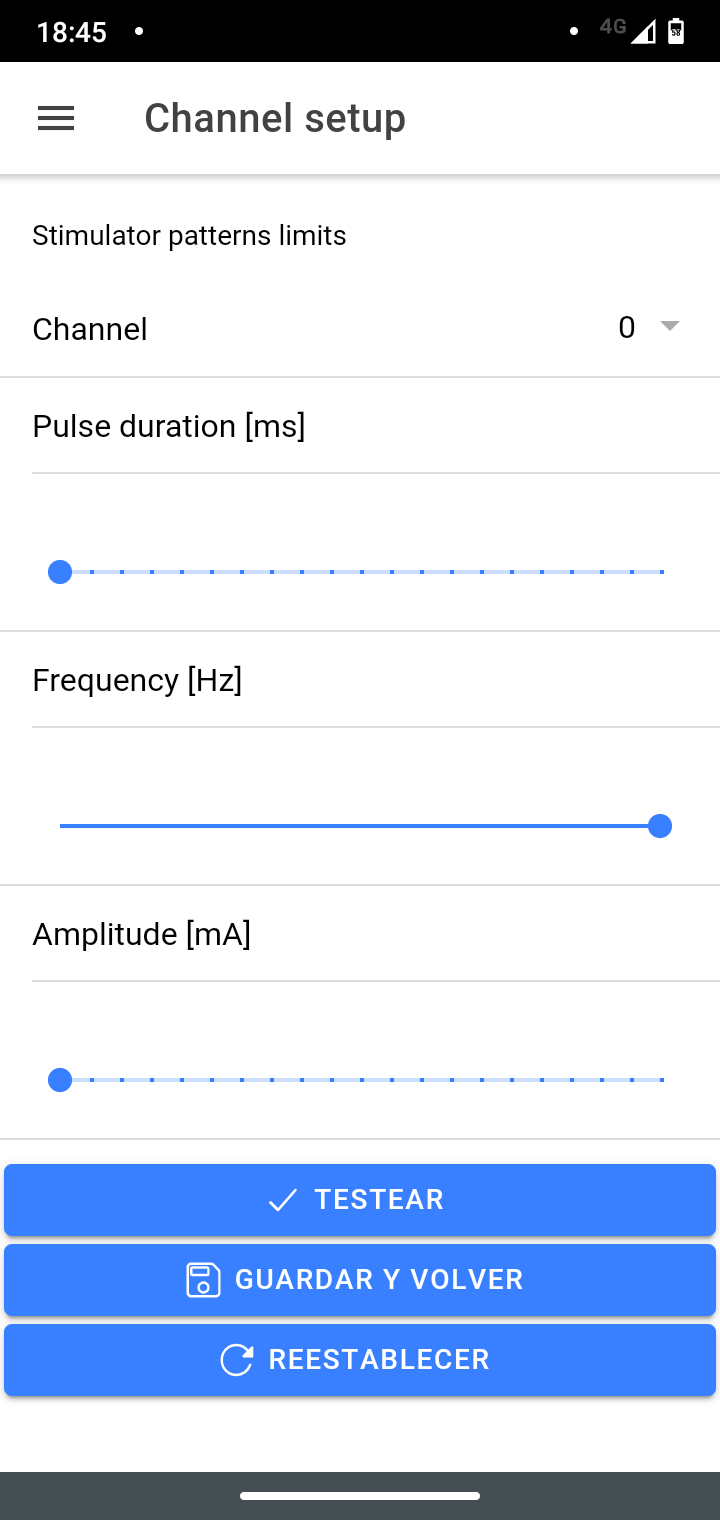
\includegraphics[width=.8\linewidth]{figs/04_ch_setup.png}
  \caption{Configuración de cada canal.}
  \label{fig:ch_setup}
\end{subfigure}
\caption{Páginas de configuración}
\label{fig:config_pages}
\end{figure}

%\section{Código fuente}

\section{Guía de evaluación}
%\begin{itemize}
%\item Aspectos a tener en cuenta:
\begin{todolist}
  \item El proyecto puede ser una integración con una api rest  (ABM de una entidad, ocupando los 4 verbos GET POST PUT DELETE) o puede ser un proyecto que utilice algún plugin de ionic native (bluetooth, geolacation, cámara de fotos, etc).
  \item El proyecto debe constar con alert de ionic para la información hacia el usuario, validaciones de datos de ingreso, ngFor o ngIf dentro del HTML y algún tipo de posicionamiento de objetos dentro de la pantalla por medio de CSS. (Estos puntos deben estar contenidos si o si dentro del proyecto)
  \item La entrega se tiene que realizar en la seccion de tareas, subiendo un pdf con una descripción básica del proyecto y un link de su github personal. El último commit debe estar realizado antes de la fecha limite dada.
  \item Fecha limite 15 de Octubre. Cualquier proyecto entregado fuera de rango no va a ser aprobado.
\end{todolist}	
	%\end{itemize}
%Use http://www.tablesgenerator.com/
